\documentclass[3p, authoryear]{elsarticle} %review=doublespace preprint=single 5p=2 column
%%% Begin My package additions %%%%%%%%%%%%%%%%%%%
\usepackage[hyphens]{url}

  \journal{Findings} % Sets Journal name


\usepackage{lineno} % add
\providecommand{\tightlist}{%
  \setlength{\itemsep}{0pt}\setlength{\parskip}{0pt}}

\usepackage{graphicx}
%%%%%%%%%%%%%%%% end my additions to header

\usepackage[T1]{fontenc}
\usepackage{lmodern}
\usepackage{amssymb,amsmath}
\usepackage{ifxetex,ifluatex}
\usepackage{fixltx2e} % provides \textsubscript
% use upquote if available, for straight quotes in verbatim environments
\IfFileExists{upquote.sty}{\usepackage{upquote}}{}
\ifnum 0\ifxetex 1\fi\ifluatex 1\fi=0 % if pdftex
  \usepackage[utf8]{inputenc}
\else % if luatex or xelatex
  \usepackage{fontspec}
  \ifxetex
    \usepackage{xltxtra,xunicode}
  \fi
  \defaultfontfeatures{Mapping=tex-text,Scale=MatchLowercase}
  \newcommand{\euro}{€}
\fi
% use microtype if available
\IfFileExists{microtype.sty}{\usepackage{microtype}}{}
\usepackage{natbib}
\bibliographystyle{apalike}
\usepackage{longtable,booktabs,array}
\usepackage{calc} % for calculating minipage widths
% Correct order of tables after \paragraph or \subparagraph
\usepackage{etoolbox}
\makeatletter
\patchcmd\longtable{\par}{\if@noskipsec\mbox{}\fi\par}{}{}
\makeatother
% Allow footnotes in longtable head/foot
\IfFileExists{footnotehyper.sty}{\usepackage{footnotehyper}}{\usepackage{footnote}}
\makesavenoteenv{longtable}
\ifxetex
  \usepackage[setpagesize=false, % page size defined by xetex
              unicode=false, % unicode breaks when used with xetex
              xetex]{hyperref}
\else
  \usepackage[unicode=true]{hyperref}
\fi
\hypersetup{breaklinks=true,
            bookmarks=true,
            pdfauthor={},
            pdftitle={Vehicle Crash Severity Correlating Factors},
            colorlinks=false,
            urlcolor=blue,
            linkcolor=magenta,
            pdfborder={0 0 0}}
\urlstyle{same}  % don't use monospace font for urls

\setcounter{secnumdepth}{5}
% Pandoc toggle for numbering sections (defaults to be off)

% Pandoc citation processing

% Pandoc header
\usepackage{booktabs}
\usepackage{booktabs}
\usepackage{longtable}
\usepackage{array}
\usepackage{multirow}
\usepackage{wrapfig}
\usepackage{float}
\usepackage{colortbl}
\usepackage{pdflscape}
\usepackage{tabu}
\usepackage{threeparttable}
\usepackage{threeparttablex}
\usepackage[normalem]{ulem}
\usepackage{makecell}
\usepackage{xcolor}



\begin{document}
\begin{frontmatter}

  \title{Vehicle Crash Severity Correlating Factors}
    \author[Brigham Young University]{Samuel Runyan\corref{1}}
   \ead{samyan@byu.edu} 
      \address[Brigham Young University]{Civil and Environmental Engineering Department, 430 Engineering Building, Provo, Utah 84602}
    
  \begin{abstract}
  Crash data from the state of Utah was analyzed to answer the question, ``what variables correlate to crash severity?''. Variables related to manner of collision, presence of schools near crashes, and presence of transit stops near crashes were considered in this analysis. It was determined that angle crashes at intersections and same-direction sideswipe crashes at roadway segments were more strongly correlated to crash severity, but the presence of schools and transit stops did not have a strong correlation to crash severity. There is a considerable correlation between pedestrian involvement and crash severity, so different variables related to pedestrian presence could be used to build a crash severity model.
  \end{abstract}
   \begin{keyword} Highway Safety Analysis Crash Severity Statistical Correlation\end{keyword}
 \end{frontmatter}

\hypertarget{intro}{%
\section{QUESTIONS}\label{intro}}

\citet{ghadi2020} attempted to determine the impact of environmental variables on crash severity, but few others have added to this research. The purpose of this article is to identify any additional factors that may correlate to crash severity such as the manner of collision, and variables related to the presence of pedestrians. The results of this article will help determine which of these variables are significant enough to include in severity-weighted network screening. In the past, many network screening models have been limited by precedent, but this research aims to expound on and improve tried and tested methods. With better understanding of how crash variables relate to crash severity, it may be possible to more proactively prevent severe crashes rather than waiting for them to happen before they can be modeled.

A major difficulty with most current network screening methodologies is that they do not account for the influence of crash severity towards the overall potential for safety improvement (PSI) of roadways. Therefore, it is valuable to use a crash severity-weighted approach when performing network screening. \citet{yasmin2018} and \citet{afghari2020} assert that a joint crash count with crash severity model is best suited to identify sites with the most PSI because of the correlation between crash counts and crash severity. As part of this joint model, it may be helpful to consider other factors which may contribute to the crash severity distribution at a given site.

\hypertarget{methods}{%
\section{METHODS}\label{methods}}

Pearson correlation factors were calculated to determine correlation to crash severity in this study. Equation \eqref{eq:pearson} shows how to calculate Pearson correlation given two potentially correlated variables, X and Y, using covariance.

\begin{equation}
  \rho = \frac{\text{cov}(X,Y)}{\sigma_x \sigma_y}
  \label{eq:pearson}
\end{equation}

Manner of collision variables and pedestrian related variables were compared to crash severity to determine correlation factors. The pedestrian related variables used here are involvment of pedestrians, pedacycle, or motorcycles in the crash as well as the presence or number of schools or transit stops within 1000 feet of the crash. The resulting correlation factors for manner of collision are shown in Table \ref{tab:Manner} and the correlation factors for pedestrian variables are shown in Table \ref{tab:Ped}. These correlation factors were evaluated at intersections and roadway segments separately to ensure homogeneity of roadway characteristics at crash locations.

\begin{table}

\caption{\label{tab:Manner}Correlation Matrix for Crash Severity and Manner of Collision}
\centering
\resizebox{\linewidth}{!}{
\begin{tabular}[t]{>{\raggedright\arraybackslash}p{5em}>{\centering\arraybackslash}p{4em}>{\centering\arraybackslash}p{4em}>{\centering\arraybackslash}p{4em}>{\centering\arraybackslash}p{4em}>{\centering\arraybackslash}p{4em}>{\centering\arraybackslash}p{4em}}
\toprule
\multicolumn{1}{c}{ } & \multicolumn{3}{c}{Segments} & \multicolumn{3}{c}{Intersections} \\
\cmidrule(l{3pt}r{3pt}){2-4} \cmidrule(l{3pt}r{3pt}){5-7}
  & Severity 5 (Fatal) & Severity 3-5 (Injury) & Total Crashes & Severity 5 (Fatal) & Severity 3-5 (Injury) & Total Crashes\\
\midrule
\cellcolor{gray!6}{\textbf{Angle}} & \cellcolor{gray!6}{0.18} & \cellcolor{gray!6}{0.60} & \cellcolor{gray!6}{0.52} & \cellcolor{gray!6}{0.26} & \cellcolor{gray!6}{0.87} & \cellcolor{gray!6}{0.90}\\
\addlinespace
\textbf{Front to Rear} & 0.14 & 0.67 & 0.88 & 0.20 & 0.68 & 0.92\\
\addlinespace
\cellcolor{gray!6}{\textbf{Head on}} & \cellcolor{gray!6}{0.30} & \cellcolor{gray!6}{0.55} & \cellcolor{gray!6}{0.48} & \cellcolor{gray!6}{0.20} & \cellcolor{gray!6}{0.64} & \cellcolor{gray!6}{0.69}\\
\addlinespace
\textbf{Sideswipe in the Same Direction} & 0.20 & 0.70 & 0.88 & 0.22 & 0.53 & 0.79\\
\addlinespace
\cellcolor{gray!6}{\textbf{Sideswipe in the Opposite Direction}} & \cellcolor{gray!6}{0.29} & \cellcolor{gray!6}{0.48} & \cellcolor{gray!6}{0.37} & \cellcolor{gray!6}{0.18} & \cellcolor{gray!6}{0.60} & \cellcolor{gray!6}{0.69}\\
\addlinespace
\textbf{Collision with Parked Vehicle} & 0.22 & 0.42 & 0.39 & 0.07 & 0.24 & 0.32\\
\addlinespace
\cellcolor{gray!6}{\textbf{Rear to Side}} & \cellcolor{gray!6}{0.09} & \cellcolor{gray!6}{0.16} & \cellcolor{gray!6}{0.15} & \cellcolor{gray!6}{0.21} & \cellcolor{gray!6}{0.16} & \cellcolor{gray!6}{0.20}\\
\addlinespace
\textbf{Rear to Rear} & 0.08 & 0.18 & 0.20 & 0.05 & 0.05 & 0.08\\
\bottomrule
\end{tabular}}
\end{table}

\begin{table}

\caption{\label{tab:Ped}Correlation Matrix for Crash Severity and Pedestrain Variables}
\centering
\resizebox{\linewidth}{!}{
\begin{tabular}[t]{>{\raggedright\arraybackslash}p{5em}>{\centering\arraybackslash}p{4em}>{\centering\arraybackslash}p{4em}>{\centering\arraybackslash}p{4em}>{\centering\arraybackslash}p{4em}>{\centering\arraybackslash}p{4em}>{\centering\arraybackslash}p{4em}}
\toprule
\multicolumn{1}{c}{ } & \multicolumn{3}{c}{Segments} & \multicolumn{3}{c}{Intersections} \\
\cmidrule(l{3pt}r{3pt}){2-4} \cmidrule(l{3pt}r{3pt}){5-7}
  & Severity 5 (Fatal) & Severity 3-5 (Injury) & Total Crashes & Severity 5 (Fatal) & Severity 3-5 (Injury) & Total Crashes\\
\midrule
\cellcolor{gray!6}{\textbf{Pedestrian Involved}} & \cellcolor{gray!6}{0.27} & \cellcolor{gray!6}{0.47} & \cellcolor{gray!6}{0.37} & \cellcolor{gray!6}{0.19} & \cellcolor{gray!6}{0.56} & \cellcolor{gray!6}{0.42}\\
\addlinespace
\textbf{Pedacycle Involved} & 0.10 & 0.33 & 0.25 & 0.12 & 0.57 & 0.37\\
\addlinespace
\cellcolor{gray!6}{\textbf{Motorcycle Involved}} & \cellcolor{gray!6}{0.31} & \cellcolor{gray!6}{0.57} & \cellcolor{gray!6}{0.46} & \cellcolor{gray!6}{0.16} & \cellcolor{gray!6}{0.60} & \cellcolor{gray!6}{0.47}\\
\addlinespace
\textbf{Number of Schools Within 1000 Feet} & -0.04 & 0.02 & 0.02 & -0.05 & -0.08 & -0.03\\
\addlinespace
\cellcolor{gray!6}{\textbf{Presence of Schools Within 1000 Feet}} & \cellcolor{gray!6}{0.01} & \cellcolor{gray!6}{0.16} & \cellcolor{gray!6}{0.14} & \cellcolor{gray!6}{-0.03} & \cellcolor{gray!6}{-0.04} & \cellcolor{gray!6}{0.01}\\
\addlinespace
\textbf{Number of Transit Stops Within 1000 Feet} & 0.00 & 0.20 & 0.16 & -0.01 & 0.19 & 0.12\\
\addlinespace
\cellcolor{gray!6}{\textbf{Presence of Transit Stops Within 1000 Feet}} & \cellcolor{gray!6}{0.00} & \cellcolor{gray!6}{0.27} & \cellcolor{gray!6}{0.30} & \cellcolor{gray!6}{0.07} & \cellcolor{gray!6}{0.32} & \cellcolor{gray!6}{0.19}\\
\bottomrule
\end{tabular}}
\end{table}

Crash data for this analysis were retrieved from the Utah Department of Transportation (UDOT) through police reports, and roadway data from the UDOT open data portal were used to identify intersections and segments on state routes. Data about the number of transit stops came from the Utah Transit Authority (UTA) and data about the number of schools came from the Utah Geospatial Resource Center (UGRC).

\hypertarget{findings}{%
\section{FINDINGS}\label{findings}}

For this study, we are mostly interested in correlation to total injury-causing crashes because these are generally considered severe, and often are or have the potential to be fatal.

The correlation between injury crashes and manner of collision are summarized in Figure \ref{fig:mannerSeverityCorr}. From this figure we notice that angle crashes at intersections and same-direction sideswipes at segments tend to be more severe than other crashes. Therefore, preventative measures should be taken to avoid these types of crashes. Front to rear crashes also appear severe on Figure \ref{fig:mannerSeverityCorr} but Table \ref{tab:Manner} shows that these have a much lower correlation to fatal crashes than total injury crashes, so we can predict that many front to rear crashes lead to less severe injuries and are not necessarily severe. However, front to rear crashes are the most common since they have the strongest correlation to total crashes, so preventing them would significantly reduce total crashes.

\begin{figure}

{\centering 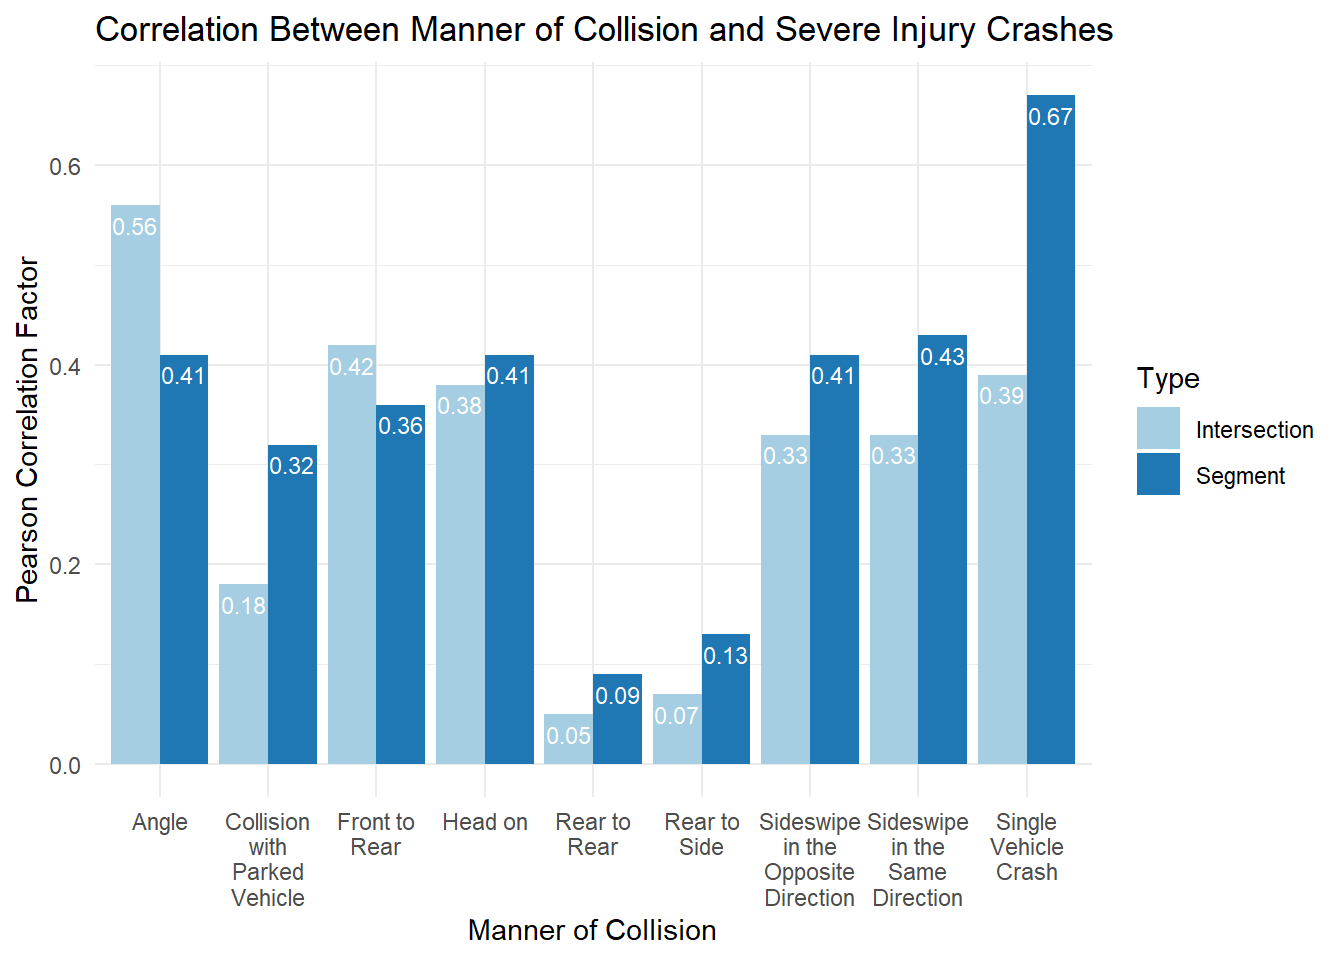
\includegraphics{Crash_Severity_Correlations_files/figure-latex/mannerSeverityCorr-1} 

}

\caption{Correlation Between Manner of Collision and Injury (Severity 3-5) Crashes}\label{fig:mannerSeverityCorr}
\end{figure}

The correlation between injury crashes and pedestrian variables are shown in Figure \ref{fig:pedSeverityCorr}. Surprisingly, there is almost no correlation between the presence of schools and severe crashes, but this may be because all schools are included. The results may change if only large schools or certain types of schools were included. The presence of transit stops also has little correlation to severe crashes and no correlation to fatal crashes, so this does not seem to be a very useful variable. The other three variables validate that there is a correlation between involvement of pedestrians, pedacyclists, and motorcyclists and crash severity, but these variables are incidental and hard to control, so more work needs to be done to determine related variables which lead to these severe pedestrian-related crashes.

\begin{figure}

{\centering 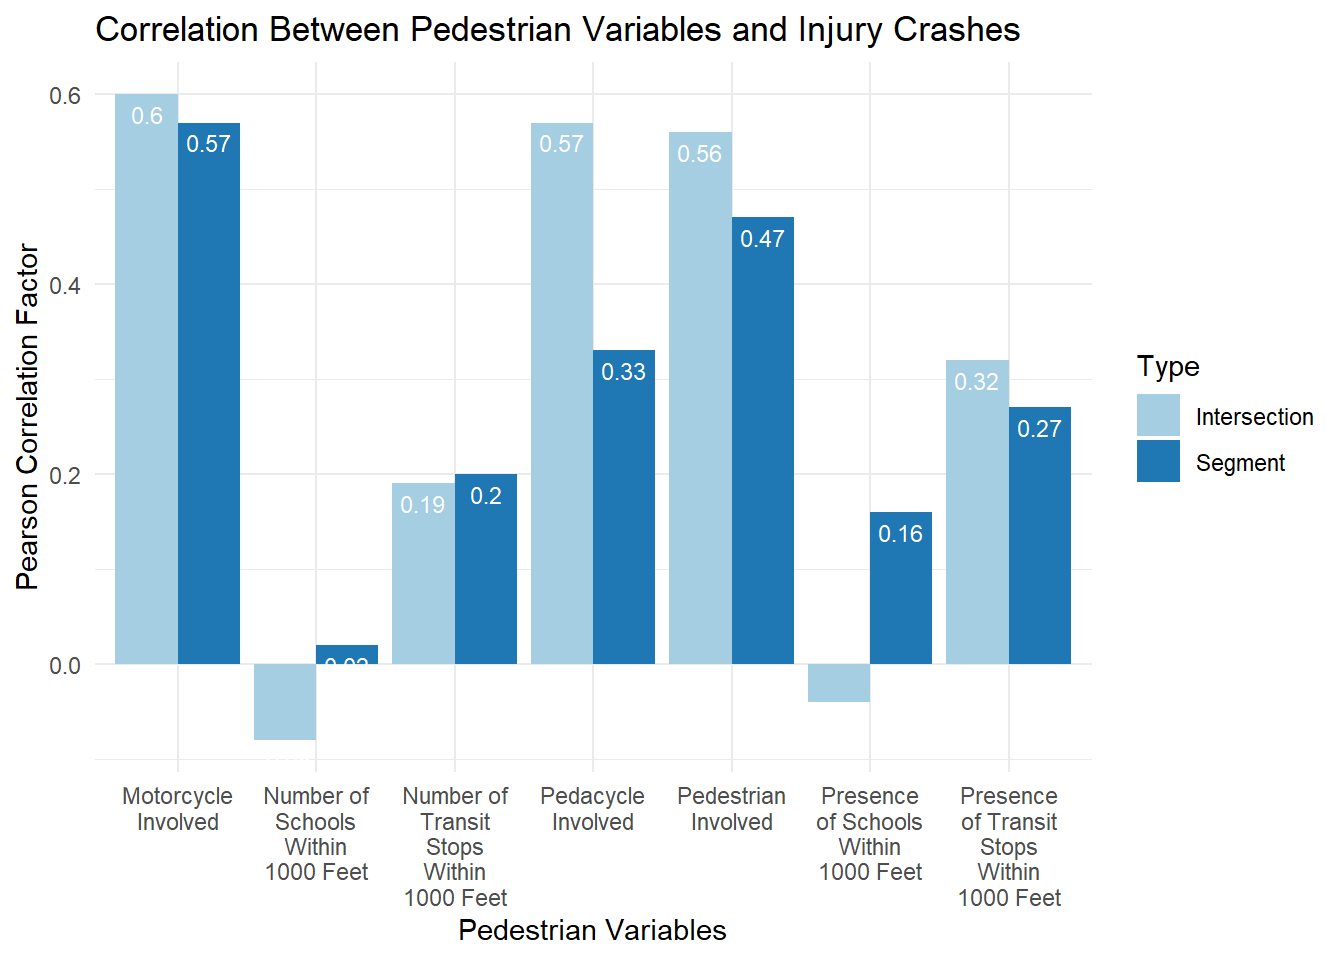
\includegraphics{Crash_Severity_Correlations_files/figure-latex/pedSeverityCorr-1} 

}

\caption{Correlation Between Pedestrian Variables and Injury (Severity 3-5) Crashes}\label{fig:pedSeverityCorr}
\end{figure}

This analysis could be used to improve severity-weighted network screening models, and implement more informed safety measures with crash severity in mind. Knowing which types of crashes are more likely to lead to severe injury will help officials design roadways and inform the public to better avoid these types of collisions. This has applications in automated vehicles as well because engineers can design vehicles to put special emphasis on avoiding the types of crashes that are more likely to lead to severe injury.

\bibliography{book.bib}


\end{document}
